\documentclass[11pt]{article}
\pagestyle{plain}
\usepackage{latexsym,exscale,amsfonts,amsmath,amssymb,array}
\usepackage{color}
\usepackage[colorlinks]{hyperref}
\setlength{\topmargin}{-2.3cm}
\setlength{\textheight}{23.8cm}
\setlength{\oddsidemargin}{-0.5cm}
\setlength{\textwidth}{17cm}
\setlength{\parindent}{0cm}
\setlength{\parskip}{.4cm}
\newcommand{\totaldiffx}{\frac{d}{dx}}
\newcommand{\pardiffx}{\frac{\partial}{\partial x}}
\newcommand{\luft}{\:\!}

\usepackage{graphicx}
\usepackage[latin1]{inputenc}
\usepackage{mathpazo}
\usepackage[T1]{fontenc}
\usepackage[comma,numbers,sort&compress]{natbib}


\begin{document}
\begin{center}
\large \bf Computational Astrophysics \rm \\
2019\\
{\small Exercises 08. Root Finding}
\end{center}

{\bf Curve Fitting: The $M_\mathrm{BH}-\sigma_*$ Relation }

The code {\tt solution8ab.py} implements the routine to read the data files using the {\tt astropy} command {\tt ascii}. The data is stored in numpy arrays. We also implemented a function to perform the linear fit in the form 
\begin{equation}
\log \left( \frac{M_{BH}}{M_{\odot }} \right) = \alpha + \beta \log \left( \frac{\sigma_{*} }{\sigma_0 }  \right)
\end{equation}
with the equations presented in class, including  data uncertainties. The reference value in the dispersion velocity is $\sigma_0 = 200 \text{ km s}^{-1}$. The linear fit function returns the coefficients $\alpha$ and $\beta$ together with the corresponding uncertainties $\sigma_{\alpha}$ and $\sigma_{\beta}$. \\

For the given data, without errors,  the $M_\mathrm{BH}-\sigma_*$ relation is given by the linear fit with parameters
\begin{eqnarray}
\alpha &=& 7.663 \pm 0.183 \\
\beta &=&  2.925 \pm 0.547,
\end{eqnarray}
which can be seen in Figure \ref{fig:noerrorfit}.

\begin{figure}[h]
\centering
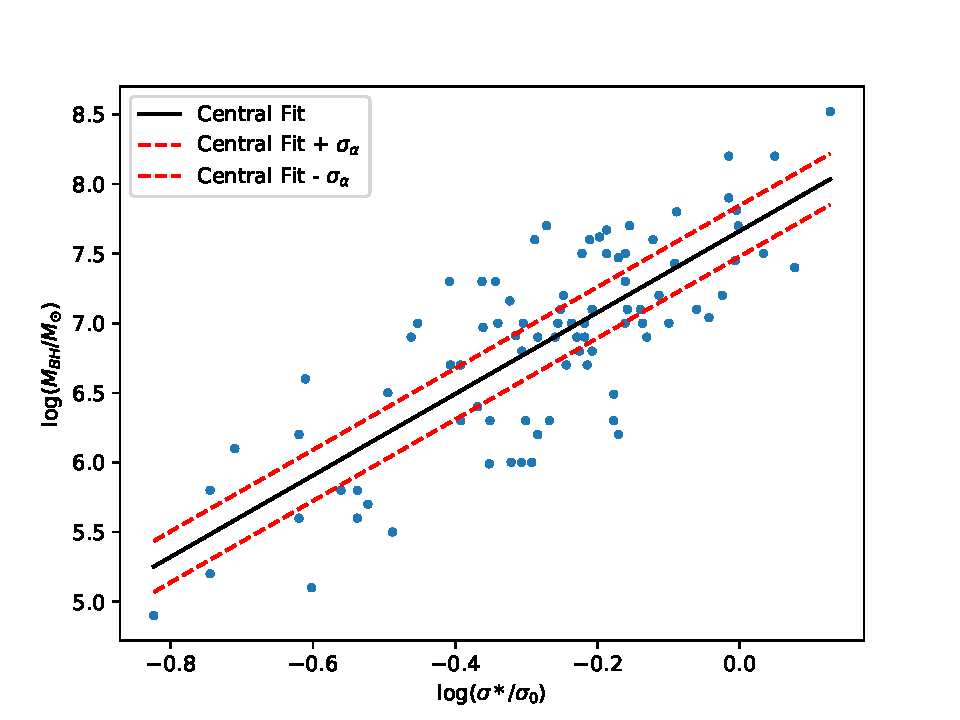
\includegraphics[scale=0.5]{M-sigma_no_error.pdf}
\caption{Linear fit without data errors.}
\label{fig:noerrorfit}
\end{figure}

In {\tt solution8c1.py} we include the error data for the black hole mass. Te resulting linear fit has the parameter
\begin{eqnarray}
\alpha &=& 7.779 \pm 0.015 \\
\beta &=&  3.232 \pm 0.061,
\end{eqnarray}
and the corresponding plot is given in Figure \ref{fig:Merrorfit}.
\begin{figure}[h]
\centering
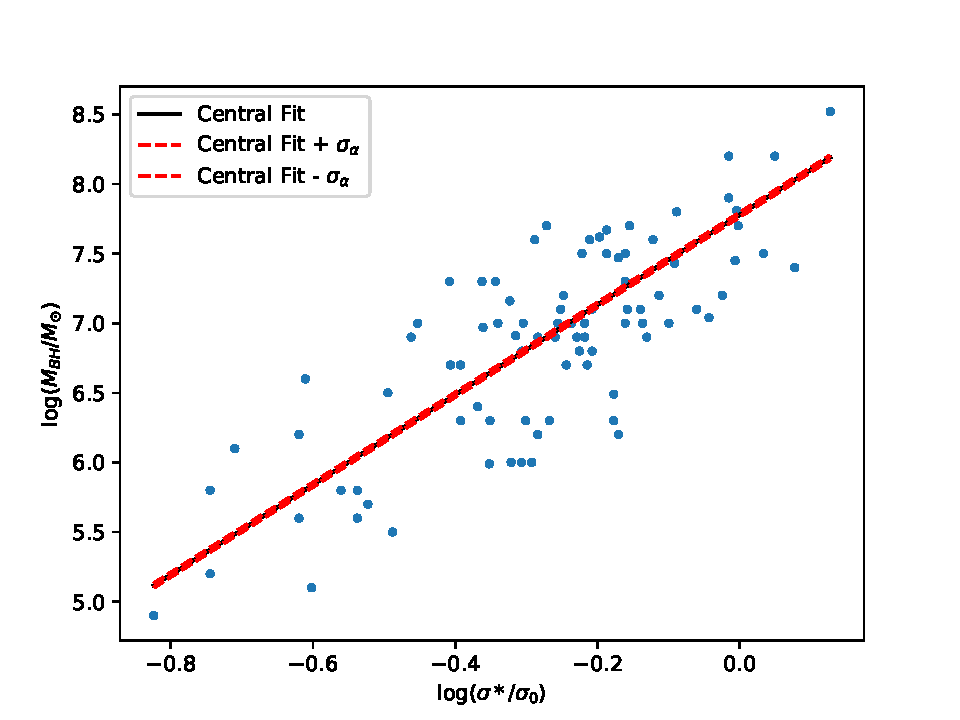
\includegraphics[scale=0.5]{M-sigma_with_errorM.pdf}
\caption{Linear fit with data error in $\log (M_{BH}/M_{\odot })$.}
\label{fig:Merrorfit}
\end{figure}

Finally, including data errors in both variables, the linear fit has the parameters
\begin{eqnarray}
\alpha &=& 7.680 \pm 1.462 \\
\beta &=&  2.912 \pm 4.917,
\end{eqnarray}
and the corresponding plot is given in Figure \ref{fig:Allerrorsfit}.
\begin{figure}[h]
\centering
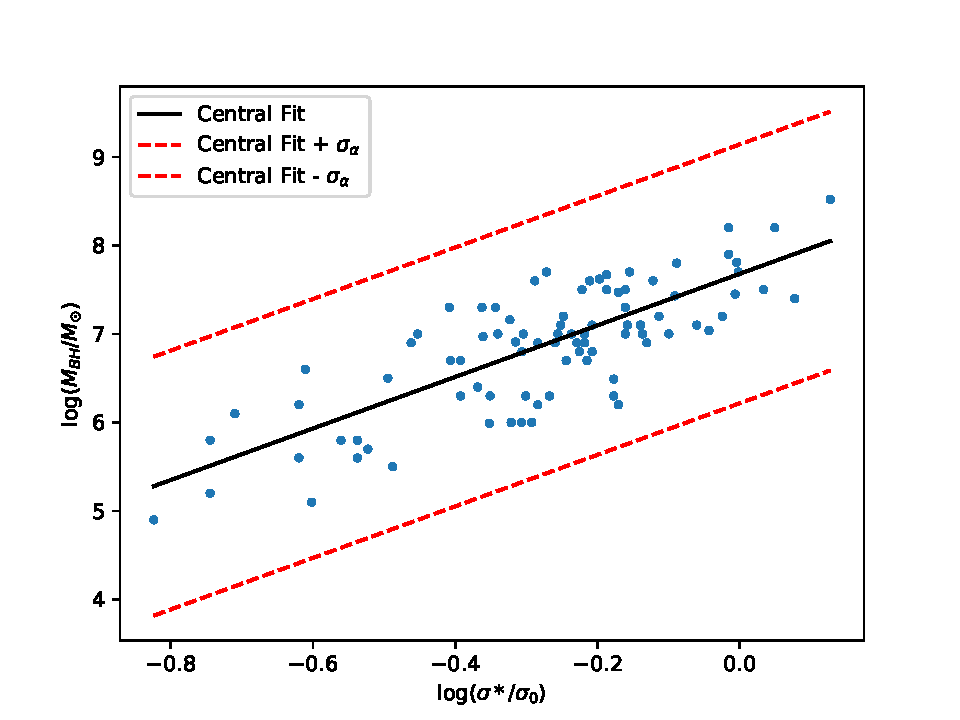
\includegraphics[scale=0.5]{M-sigma_with_errors.pdf}
\caption{Linear fit with data errors in $\log (M_{BH}/M_{\odot })$ and $\sigma_{*}$.}
\label{fig:Allerrorsfit}
\end{figure}

\end{document}

